\documentclass{beamer}
 
\usepackage[utf8]{inputenc}
\usepackage[T1]{fontenc}
\usetheme{Copenhagen}
\usepackage{listings,xcolor}
\usepackage{xcolor}


\title{Server Side GraphQL}
\subtitle{Using Elixir, Phoenix and Absinthe}

\author[rlb3]{Robert Boone}
\institute[C1]{ChaiOne}
\date{June 27, 2018}
\logo{
\includegraphics[height=1.0cm]{absinthe-logo}} 
 
 
\begin{document}

\lstdefinelanguage{elixir}{
    morekeywords={case,catch,def,do,else,false,%
        use,alias,receive,timeout,defmacro,defp,%
        for,if,import,defmodule,defprotocol,%
        nil,defmacrop,defoverridable,defimpl,%
        super,fn,raise,true,try,end,with,%
        unless},
    otherkeywords={<-,->, |>, \%\{, \}, \{, \, (, )},
    sensitive=true,
    morecomment=[l]{\#},
    morecomment=[n]{/*}{*/},
    morecomment=[s][\color{purple}]{:}{\ },
    morestring=[s][\color{orange}]"",
    commentstyle=\color{purple},
    keywordstyle=\color{blue},
    stringstyle=\color{red},
	basicstyle=\ttfamily,
	breaklines,
	showstringspaces=false,
	frame=tb
}

\defverbatim[colored]\CustomScalarType{
  \begin{lstlisting}[language=elixir, caption={Custom Scaler Type}, captionpos=b, basicstyle=\tiny]
  scalar :date do
    parse(fn input ->
      case Timex.parse!(input.value, "{YYYY}-{0M}-{D}") |> DateTime.from_naive("Etc/UTC") do
        {:ok, date} -> {:ok, date}
        _ -> :error
      end
    end)

    serialize(fn date -> Date.to_iso8601(date) end)
  end
  \end{lstlisting}
}

\defverbatim[colored]\EnumType{
  \begin{lstlisting}[language=elixir, caption={Enum Type}, captionpos=b, basicstyle=\tiny]
    enum :priority_level, description: "Todo priority levels" do
      value :high, as: :true, description: "High Priority"
      value :low, as: :false, description: "Low Priority"
    end
  \end{lstlisting}
}

\defverbatim[colored]\ObjectType{
  \begin{lstlisting}[language=elixir, caption={Object Type}, captionpos=b, basicstyle=\tiny]
  object :todo do
    field(:id, :id, description: "Todo id")
    field(:title, :string, description: "Todo Title")
    field(:priority, :priority_level, description: "Priority?")
    field(:due_at, :date, description: "Due date")
    field(:complete, :boolean, description: "Todo complete")
  end
  \end{lstlisting}
}

\defverbatim[colored]\RootObjectType{
  \begin{lstlisting}[language=elixir, caption={User Root Object Type},
captionpos=b, basicstyle=\tiny]
    query do
      field :users, list_of(:user), description: "List users in my groups" do
        resolve(&FariWeb.Resolvers.Users.list_users/3)
      end
    end
  \end{lstlisting}
}

\defverbatim[colored]\Resolver{
  \begin{lstlisting}[language=elixir, caption={Resolve function}, captionpos=b, basicstyle=\tiny]
    def list_users(_obj, _args, %{context: %{current_user: user}}) do
      users =
        user
        |> Fari.Repo.preload(:groups)
        |> get_groups()
        |> Enum.map(fn group -> Fari.Repo.preload(group, :users) end)
        |> Enum.map(fn g -> g.users end)
        |> List.flatten()

      {:ok, users}
  end

  \end{lstlisting}
}

\defverbatim[colored]\Module{
  \begin{lstlisting}[language=elixir, caption={Module}, captionpos=b, basicstyle=\tiny]
  
  defmodule Core do
    def add(a,b) do
      a + b
    end
  end
  
  Core.add(1,1) == 2
  
  add = fn(a,b) -> a + b end
  add.(1,1) == 2
  
  \end{lstlisting}
}

\defverbatim[colored]\PatternMatching{
  \begin{lstlisting}[language=elixir, caption={Pattern Matching}, captionpos=b, basicstyle=\tiny]
  defmodule Core do
    def email(%User{name: name, email: email} = user) do
      IO.puts("#{name}'s email is #{email}.")
      user
    end
    
    def email(%Admin{} = admin) do
      IO.puts("admin@example.com")
      admin
    end
  end
  
  email =
    fn
      (%User{email: email} = user) -> "#{user.name}'s email is #{email}"
      (%Admin{})                   -> "admin@example.com"
    end
          
  email.(user)
  \end{lstlisting}
}

\defverbatim[colored]\EnumModule{
\begin{verbatim}
    Enum.__info__(:functions) |> length
    96
  \end{verbatim}
}

\defverbatim[colored]\ErlangPipe{
  \begin{verbatim}
    four(three(two(one(x), global: false)))
    
    x1 = one(x)
    x2 = two(x1, global: false)
    x3 = three(x2)
    x4 = four(x3)
  \end{verbatim}
}

\defverbatim[colored]\Pipes{
  \begin{verbatim}
    String.upcase("hello world")
    "HELLO WORLD"

    "hello world" |> String.upcase()
    "HELLO WORLD"
  \end{verbatim}
}

\defverbatim[colored]\PipesTwo{
  \begin{verbatim}    
    x
    |> one()
    |> two(global: false)
    |> three()
    |> four()
  \end{verbatim}
}

\defverbatim[colored]\ForComp{
  \begin{lstlisting}[language=elixir, caption={For Comprehension}, captionpos=b, basicstyle=\tiny]
      alias :lists, as: Lists
      alias :math, as: Math
 
      for a <- Lists.seq(1,100),
          b <- Lists.seq(1,100),
          c <- Lists.seq(1,100),
          Math.pow(a,2) + Math.pow(b,2) == Math.pow(c, 2),
        do: [a: a, b: b, c: c]
  

      [
        [a: 3, b: 4, c: 5],
        [a: 4, b: 3, c: 5],
        [a: 5, b: 12, c: 13],
        [a: 6, b: 8, c: 10],
        ...
      ]
  \end{lstlisting}
}
\defverbatim[colored]\ForCompTwo{
\begin{lstlisting}[language=elixir, caption={For Comprehension}, captionpos=b, basicstyle=\tiny]
  for x <- [1,2,3], into: %{} do
    {x, x+10}
  end
  
  %{1 => 11, 2 => 12, 3 => 13}
\end{lstlisting}
}

\defverbatim[colored]\Using{
\begin{lstlisting}[language=elixir, caption={Using Macro}, captionpos=b, basicstyle=\tiny]
  defmodule FariWeb do
    def controller do
      quote do
        use Phoenix.Controller, namespace: FariWeb
        import Plug.Conn
        import FariWeb.Router.Helpers
        import FariWeb.Gettext
      end
    end
  
    defmacro __using__(which) when is_atom(which) do
      apply(__MODULE__, which, [])
    end
  end
  
  defmodule FariWeb.UserController do
    use FariWeb, :controller
  end
\end{lstlisting}
}

\defverbatim[colored]\WithMacro{
\begin{lstlisting}[language=elixir, caption={With Macro}, captionpos=b, basicstyle=\tiny]
  def login(_obj, args, _ctx) do
    user = Repo.get_by(User, email: args.email)

    with {:ok, user} <- Comeonin.Argon2.check_pass(user, args.password),
         {:ok, token, _claims} <- Fari.Guardian.encode_and_sign(user) do
      {:ok, %{token: token}}
    else
      {:error, "invalid password"} ->
        {:error, "Bad Username or password"}

      {:error, message} ->
        {:error, message}
    end
  end
\end{lstlisting}
}

\defverbatim[colored]\ModulePlug{
\begin{lstlisting}[language=elixir, caption={Using Macro}, captionpos=b, basicstyle=\tiny]
defmodule ContexthubWeb.Auth do
  use ContexthubWeb, :controller

  def init(opts), do: opts

  def call(conn, _opts) do
    ["Bearer " <> token] = get_req_header(conn, "authorization")
    case Guardian.decode_and_verify(token) do
      {:ok, _claims} -> assign(conn, :authenticated, true)
      {:error, _reason} ->
        conn
        |> put_status(401)
        |> json(%{error: "unauthenticated"})
        |> halt
    end
  end
end

defmodule ContexthubWeb.NotificationController do
  plug ContexthubWeb.Auth
end
\end{lstlisting}
}

\defverbatim[colored]\FunctionPlug{
\begin{lstlisting}[language=elixir, caption={Using Macro}, captionpos=b, basicstyle=\tiny]
  defp resource(conn, _opt) do
    with {:ok, user} <- Fari.Auth.resource_from_token(conn) do
      conn
      |> Plug.Conn.put_private(:absinthe, %{context: %{current_user: user}})
    else
      {:error, :token_expired} ->
        conn
        |> Plug.Conn.put_private(:absinthe, %{context: %{token_expired: true}})

      error ->
        IO.inspect(error)
        conn
    end
  end
  
  plug(:resource)
\end{lstlisting}
}
\defverbatim[colored]\InputTypeDef{
\begin{lstlisting}[language=elixir, caption={Input Types}, captionpos=b, basicstyle=\tiny]
@desc "Filtering options for the menu item list"
input_object :menu_item_filter do
  @desc "Matching a name"
  field :name, :string

  @desc "Matching a category name"
  field :category, :string
  
  @desc "Matching a tag"
  field :tag, :string
  
  @desc "Priced above a value"
  field :priced_above, :float
  
  @desc "Priced below a value"
  field :priced_below, :float
end
\end{lstlisting}
}

\defverbatim[colored]\InputTypeApl{
\begin{lstlisting}[language=elixir, caption={Input Types}, captionpos=b, basicstyle=\tiny]
field :menu_items, list_of(:menu_item) do
  arg :filter, :menu_item_filter
  arg :order, type: :sort_order, default_value: :asc
  resolve &Resolvers.Menu.menu_items/3
end
\end{lstlisting}
}

\defverbatim[colored]\Sub{
\begin{lstlisting}[language=elixir, caption={Subscriptions}, captionpos=b, basicstyle=\tiny]
  subscription do
    field :marked_todo, :todo do
      config(fn _args, _info ->
        {:ok, topic: "*"}
      end)

      resolve(fn todo, _, _ ->
        {:ok, todo}
      end)
    end
  end
  
  defp notify_mark({:ok, todo}) do
    Absinthe.Subscription.publish(FariWeb.Endpoint, todo, marked_todo: "*")
    {:ok, todo}
  end
\end{lstlisting}
}

\defverbatim[colored]\Mid{
\begin{lstlisting}[language=elixir, caption={Authentication}, captionpos=b, basicstyle=\tiny]
  def middleware(middleware, %Field{identifier: id}, _object) when id in [:register, :login] do
    middleware
  end

  def middleware(middleware, _field, %Object{identifier: id}) when id in [:query, :mutation] do
    [Fari.Authentication | middleware]
  end

  def middleware(middleware, _field, _object) do
    middleware
  end
}
\end{lstlisting}
}

\defverbatim[colored]\Auth{
\begin{lstlisting}[language=elixir, caption={Authentication}, captionpos=b, basicstyle=\tiny]
defmodule Fari.Authentication do
  @behaviour Absinthe.Middleware
  @moduledoc false

  def call(resolution, config) do
    case resolution.context do
      %{current_user: _} ->
        resolution

      %{token_expired: true} ->
        resolution
        |> Absinthe.Resolution.put_result({:error, "token expired"})

      _ ->
        resolution
        |> Absinthe.Resolution.put_result({:error, "unauthenticated"})
    end
  end
end
\end{lstlisting}
}

\defverbatim[colored]\SchemaDataLoader{
\begin{lstlisting}[language=elixir, caption={Data Loader}, captionpos=b, basicstyle=\tiny]
  def dataloader() do
    Dataloader.new()
    |> Dataloader.add_source(Fari.Core.User, Fari.Core.data())
    |> Dataloader.add_source(Fari.Core.Todo, Fari.Core.data())
  end

  def context(ctx) do
    Map.put(ctx, :loader, dataloader())
  end

  def plugins do
    [Absinthe.Middleware.Dataloader | Absinthe.Plugin.defaults()]
  end

\end{lstlisting}
}

\defverbatim[colored]\CoreDataLoader{
\begin{lstlisting}[language=elixir, caption={Data Loader}, captionpos=b, basicstyle=\tiny]
defmodule Fari.Core do
  alias Fari.Repo
  import Ecto.Query

  def data() do
    Dataloader.Ecto.new(Repo, query: &query/2)
  end

  # def query(Fari.Core.Todo, _args) do
  #   from(t in Fari.Core.Todo, where: t.complete == ^false)
  # end

  def query(queryable, _args) do
    queryable
  end
end
\end{lstlisting}
}


\defverbatim[colored]\ObjectDataLoader{
 \begin{lstlisting}[language=elixir, caption={Data Loader}, captionpos=b, basicstyle=\tiny]
  object :user do
    field(:id, :id, description: "User ID")
    field(:email, :string, description: "Email")
    field(:first_name, :string, description: "First Name")
    field(:last_name, :string, description: "Last Name")

    field :full_name, :string, description: "Full name" do
      resolve(fn user, _, _ ->
        {:ok, "#{user.first_name} #{user.last_name}"}
      end)
    end

    field(
      :groups,
      list_of(:group),
      description: "User Groups",
      resolve: dataloader(Fari.Core.User, :groups)
    )

    field(
      :todos,
      list_of(:todo),
      description: "User todos",
      resolve: dataloader(Fari.Core.Todo, :todos)
    )
  end

\end{lstlisting}
}

\defverbatim[colored]\Mut{
 \begin{lstlisting}[language=elixir, caption={Mutations}, captionpos=b, basicstyle=\tiny]
    mutation do
      field :login, non_null(:session) do
        arg(:email, :string, description: "User's email")
        arg(:password, :string, description: "Password")

        resolve(&FariWeb.Resolvers.Users.login/3)
      end
    end

\end{lstlisting}
}

\begin{frame}
  \titlepage
\end{frame}

\begin{frame}
\frametitle{Table of Contents}
\tableofcontents
\end{frame}

\section{Elixir}

\begin{frame}
\frametitle{Elixir}

Elixir is a \alert{functional}, \alert{concurrent}, general-purpose programming language that runs on the Erlang virtual machine (BEAM). Elixir builds on top of Erlang and shares the same abstractions for building \alert{distributed}, \alert{fault-tolerant} applications. Elixir also provides a productive tooling and an extensible design. The latter is supported by compile-time metaprogramming with macros and polymorphism via protocols.

\end{frame}
\begin{frame}
\frametitle{Syntax}

\begin{itemize}
\item{Pipe Operator}
\item{With Macro}
\item{Modules and Functions}
\item{Pattern Matching}
\item{Enum Module}
\item{For Comprehension}
\item{Use}
\end{itemize}
\end{frame}

\begin{frame}
  \frametitle{Pipe Operator}
  
  \begin{itemize}
    \item{One aspect of functional programming is composing functions.} \pause
    \item{You compose functions by passing the output of one function as the input of the next.} \pause
    \item{By doing this you can make pipe lines of functions that transforms the data that is passed to it.}
  \end{itemize}
\end{frame}

\begin{frame}
  \frametitle{Pipe Operator}
  Without the Pipe Operator function composition can look like this:
  \rule{10.8cm}{0.4pt}
  \ErlangPipe
\end{frame}

\begin{frame}
  \frametitle{Pipe Operator}
  \Pipes
\end{frame}

\begin{frame}
  \frametitle{Pipe Operator}
  \PipesTwo
\end{frame}

\begin{frame}
\frametitle{Modules and Functions}
\Module
\end{frame}

\begin{frame}
\frametitle{Pattern Matching}

\PatternMatching
\end{frame}

\begin{frame}
  \frametitle{Enum Module}
  \EnumModule
  \begin{block}{Common Functions}
    \begin{itemize}
      \item{each}
      \item{map}
      \item{filter}
      \item{reduce}
    \end{itemize}
  \end{block}
\end{frame}

\begin{frame}
  \frametitle{With Macro}
  Another way to tackle function composition:
  \WithMacro
\end{frame}

\begin{frame}
  \frametitle{For Comprehension}
  \ForComp
\end{frame}

\begin{frame}
  In most languages this feature is called a list comprehension. The Elixir version can return other types.
  \frametitle{For Comprehension}
  \ForCompTwo
\end{frame}

\begin{frame}
  \frametitle{Using Macro}
  \Using
\end{frame}

\section{Phoenix}

\begin{frame}
\frametitle{Mix}
Mix is a build tool that provides tasks for creating, compiling, and testing Elixir projects, managing its dependencies, and more.

\begin{itemize}
\item{For those familiar with ruby mix is like:}
\begin{itemize}
\item{bundler}
\item{rake}
\item{rails CLI}
\end{itemize}
\end{itemize}
\end{frame}

\begin{frame}
\frametitle{Plug}
Plug is: \pause

\begin{itemize}
\item{Connection adapters for different web servers in the Erlang VM.} \pause
\item{A specification for composable modules between web applications.}
\end{itemize}
\end{frame}

\begin{frame}
\frametitle{Plug.Conn}
  The Plug.Conn is the main data structure. It is used to represent the \alert{Requests} and create \alert{Responses}.
\end{frame}

\begin{frame}
  \frametitle{Request fields}

  \begin{flushleft}
  \tiny
  \begin{tabular}{|r|p{3.5in}|}
  \hline
  \textbf{Name} & \textbf{Description} \\ \hline
  host          & The requested host as a binary, example: "www.example.com" \\
  path\_info    & The path split into segments, example: ["hello", "world"] \\
  request\_path & The requested path, example: /trailing/and//double//slashes/ \\
  port          & The requested port as an integer, example: 80 \\
  remote\_ip    & The IP of the client, example: \{151, 236, 219, 228\}. This field is meant to be overwritten by plugs that understand e.g. the X-Forwarded-For header or HAProxy’s PROXY protocol. It defaults to peer’s IP \\
  req\_headers  & The request headers as a list, example: [{"content-type", "text/plain"}]. Note all headers will be downcased \\
  scheme        & The request scheme as an atom, example: :http \\
  query\_string & The request query string as a binary, example: "foo=bar" \\ \hline
  \end{tabular}
  \end{flushleft}
\end{frame}

\begin{frame}
\frametitle{Fetchable fields}
\begin{flushleft}
  \tiny
  \begin{tabular}{|r|p{3.5in}|}
  \hline
  \textbf{Name} & \textbf{Description} \\ \hline
  cookies       & The request cookies with the response cookies \\
  body\_params  & The request body params, populated through a Plug.Parsers parser. \\
  query\_params & The request query params, populated through fetch\_query\_params/2 \\
  path\_params  & The request path params, populated by routers such as Plug.Router \\
  params        & The request params, the result of merging the :body\_params and :query\_params with :path\_params \\
  req\_cookies  & The request cookies (without the response ones) \\\hline
  \end{tabular}
\end{flushleft}
\end{frame}

\begin{frame}
\frametitle{Response fields}
\begin{flushleft}
  \tiny
  \begin{tabular}{|r|p{3.5in}|}
    \hline
    \textbf{Name}  & \textbf{Description} \\ \hline
     resp\_body    & The response body, by default is an empty string. It is set to nil after the response is sent, except for test connections. \\
     resp\_charset & The response charset, defaults to “utf-8” \\
     resp\_cookies & The response cookies with their name and options \\
     resp\_headers & The response headers as a list of tuples, by default cache \& control is set to "max-age=0, private, must-revalidate". Note, response headers are expected to have lower-case keys. \\
     status        & The response status \\ \hline
     
  \end{tabular}
\end{flushleft}

\end{frame}

\begin{frame}
\frametitle{Connection fields}
\begin{flushleft}
  \tiny
  \begin{tabular}{|r|p{3.5in}|}
    \hline
    \textbf{Name}  & \textbf{Description} \\ \hline
       assigns & Shared user data as a map \\
       owner & The Elixir process that owns the connection \\
       halted & The boolean status on whether the pipeline was halted \\
secret\_key\_base & A secret key used to verify and encrypt cookies. the field must be set manually whenever one of those features are used. This data must be kept in the connection and never used directly, always use Plug.Crypto.KeyGenerator.generate/3 to derive keys from it \\
state & The connection state \\ \hline

\end{tabular}
\end{flushleft}
\end{frame}

\begin{frame}
\frametitle{Private fields}

\begin{flushleft}
  \tiny
  \begin{tabular}{|r|p{3.5in}|}
  \hline
  \textbf{Name} & \textbf{Description} \\ \hline
    
    adapter & Holds the adapter information in a tuple \\
    private & Shared library data as a map \\ \hline

  \end{tabular}
\end{flushleft}



\end{frame}

\begin{frame}
\frametitle{Module Plug}
\ModulePlug
\end{frame}

\begin{frame}
\frametitle{Function Plug}
\FunctionPlug
\end{frame}


\begin{frame}
\frametitle{Channels}
Channels provide a means for bidirectional communication from clients that integrate with the Phoenix.PubSub layer for \alert{soft-realtime} functionality.

\begin{itemize}
\item{Phoenix.Transports.WebSocket}
\item{Phoenix.Transports.LongPoll}
\end{itemize}
\end{frame}

\begin{frame}
\frametitle{Channels}
You can write your own transports. Examples are:

\begin{itemize}
\item{WebRTC}
\item{Jabber}
\item{RabbitMQ}
\end{itemize}
\end{frame}

\section{GraphQL / Absinthe}

\begin{frame}
\frametitle{What is GraphQL?}
GraphQL is a data \alert{query language} developed by Facebook in 2012 and release in 2015.
\end{frame}

\begin{frame}
  \frametitle{Definition}
  \begin{description}
    \item[{Query Language}] A language for the specification of procedures for the retrieval (and sometimes also modification) of information from a database. \pause
  \end{description}
  \begin{itemize}
    \item{The fact that GraphQL can be used as a web API is an implementation detail.}
  \end{itemize}

\end{frame}

\begin{frame}
  \frametitle{Documentation}
  
  Descriptions can be added to every field:
  \ObjectType
\end{frame}

\begin{frame}
  \frametitle{Documentation - GraphiQL}
  \begin{center}
    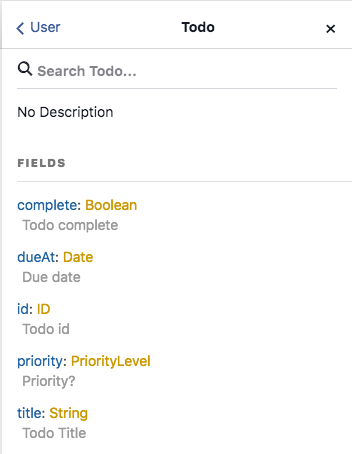
\includegraphics[width=0.5\textwidth]{todo_docs}
  \end{center}
\end{frame}

\begin{frame}
  \frametitle{Types}

  \begin{itemize}
    \item{APIs in GraphQL are organized by types and fields.}
  \end{itemize}
  \begin{block}{Builtin Types}
    \begin{itemize}
    \item{boolean}
    \item{float}
    \item{id}
    \item{integer}
    \item{string}
    \end{itemize}
  \end{block}
\end{frame}

\begin{frame}
  \frametitle{Custom Types}

  \begin{itemize}
    \item{You can also create custom Scalar Types.}
  \end{itemize}

  \CustomScalarType
\end{frame}

\begin{frame}
  \frametitle{Enum Types}
  Enum types represents one of a finite set of possible values.
  \EnumType
  
  \centering
  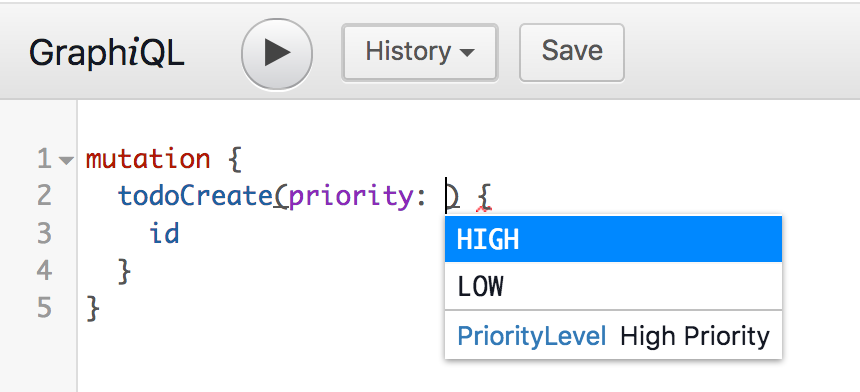
\includegraphics[width=0.5\textwidth]{graphiql-enum}
\end{frame}

\begin{frame}
  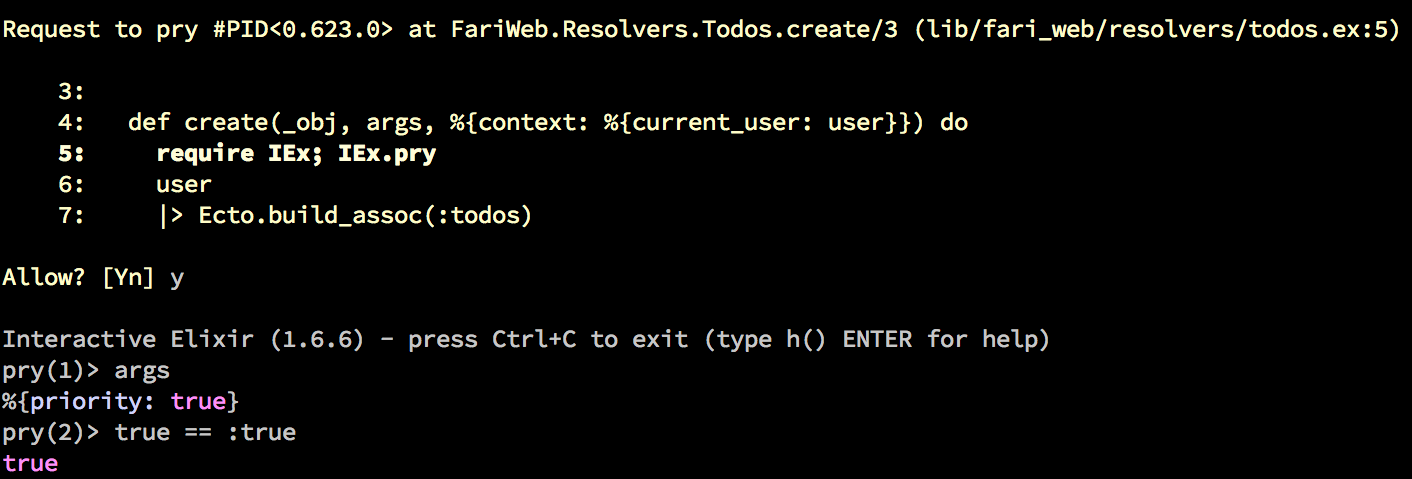
\includegraphics[width=1.0\textwidth]{enum_example}
\end{frame}

\begin{frame}
  \frametitle{Input Types}
   Input types defines a set of input fields; the input fields are either scalars, enums, or other input objects. This allows arguments to accept arbitrarily complex values.
   \InputTypeDef
\end{frame}

\begin{frame}
  \frametitle{Input Types}

   \InputTypeApl
\end{frame}

\begin{frame}
  \frametitle{Object Types}

 Objects types represent a list of named fields, each of which yields a value of a specific type.

  \ObjectType
  \end{frame}

\begin{frame}
  \frametitle{Query}

  \begin{itemize}
  \item{The Query Root object is where all queries are found.}
  \end{itemize}

  \RootObjectType

\end{frame}

\begin{frame}
  \frametitle{Resolvers}

  \begin{itemize}
    \item{The resolve function tells the object how to get it's data.}
  \end{itemize}

  \Resolver
\end{frame}

\begin{frame}
  \frametitle{Resolver Arguments}

  \begin{itemize}
  \item{Resolve functions take 3 arguments.} \pause
  \item{parent}
    \begin{itemize}
    \item{This is the object above the current object.}
    \item{At the root level this is normally nil.}\pause
    \end{itemize}
  \item{arguments} \pause
    \begin{itemize}
      \item{A map of the arguments} \pause
    \end{itemize}
  \item{Absinthe.Resolution Struct} \pause
    \begin{itemize}
      \item{This contains the \textbf{context} and other execution data}
    \end{itemize}
  \end{itemize}

\end{frame}

\begin{frame}
  \frametitle{Resolvers Return Value}

  \begin{itemize}
    \item{To have \alert{successful} result, return a tuple in the form of \texttt{\{:ok, value\}}}
    \item{To have an \alert{error} result, return a tuple in the form of \texttt{\{:error, reason\}}}
  \end{itemize}

\end{frame}

\begin{frame}
\frametitle{Mutations}

Mutations work the same way Queries do. The difference is side-effects are expected.
\Mut
\end{frame}

\begin{frame}
\frametitle{Subscriptions}

Subscriptions allow users to request data updates.

\Sub
\end{frame}

\begin{frame}
\frametitle{Authentication}

\FunctionPlug
\end{frame}

\begin{frame}
\frametitle{Authentication}

\Auth
\end{frame}

\begin{frame}
\frametitle{Authentication}

\Mid
\end{frame}

\begin{frame}
\frametitle{Data Loader}
\SchemaDataLoader
\end{frame}


\begin{frame}
\frametitle{Data Loader}

\CoreDataLoader
\end{frame}

\begin{frame}
\frametitle{Data Loader}

\ObjectDataLoader
\end{frame}

\begin{frame}
\frametitle{Questions}

\includegraphics[width=1.0\textwidth]{fari}
\end{frame}

\begin{frame}
\frametitle{Thank you}
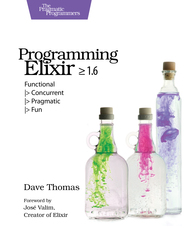
\includegraphics[width=.33\textwidth]{elixir16}

\includegraphics[width=.33\textwidth]{phoenix14}
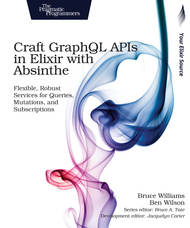
\includegraphics[width=.33\textwidth]{wwgraphql}
\end{frame}

\end{document}



